\chapter{Projektidee}

\renewcommand{\kapitelautor}{}

Die Idee des Projektes, ist die Entwicklung eines innovativen Logistiksystems in der Gastronomiebranche, das durch Verwendung von Multicoptern umgesetzt wird.
Optional wird ein Event namens ‘Fluorescent Bakery’ durchgeführt, bei dem das System zum Einsatz kommt.

Im Restaurant setzt sich jeder Gast auf seinen Platz. Anschließend können die Gäste auf Tablets, welche sich auf jedem Tisch befinden, Speisen und Getränke bestellen. Die Bestellungen werden an einen Server geschickt. Der Server schickt die Daten an ein, für Personal zugängliches Tablet und zeigt die Bestellungen und die dazugehörige Tischinformation an.

Der weitere Ablauf besteht darin, dass ein Kellner die bestellte Speise in die vorgefertigte Befestigung auf dem Multicopter stellt. Danach wählt er in einem Programm aus, um wessen Bestellung es sich handelt. Sobald der Kellner auf den „Bestellung ausliefern“-Button drückt, sendet der Server die Tischinformation an den Multicopter.

Der Multicopter fliegt autonom zum ausgewählten Tisch und landet auf einer Plattform, die er mithilfe eines geeigneten Positionierungssystems findet. Er fliegt dabei nur auf den vorgesehenen, für Besucher als gesperrt gekennzeichneten Wegen, was das Überfliegen von Menschen verhindert.

An der Plattform angekommen, legt der Multicopter die Speise ab und fliegt zurück zu seinem Stützpunkt (Base).
\section{Ablauf}

\begin{figure}[tbh]
\begin{centering}
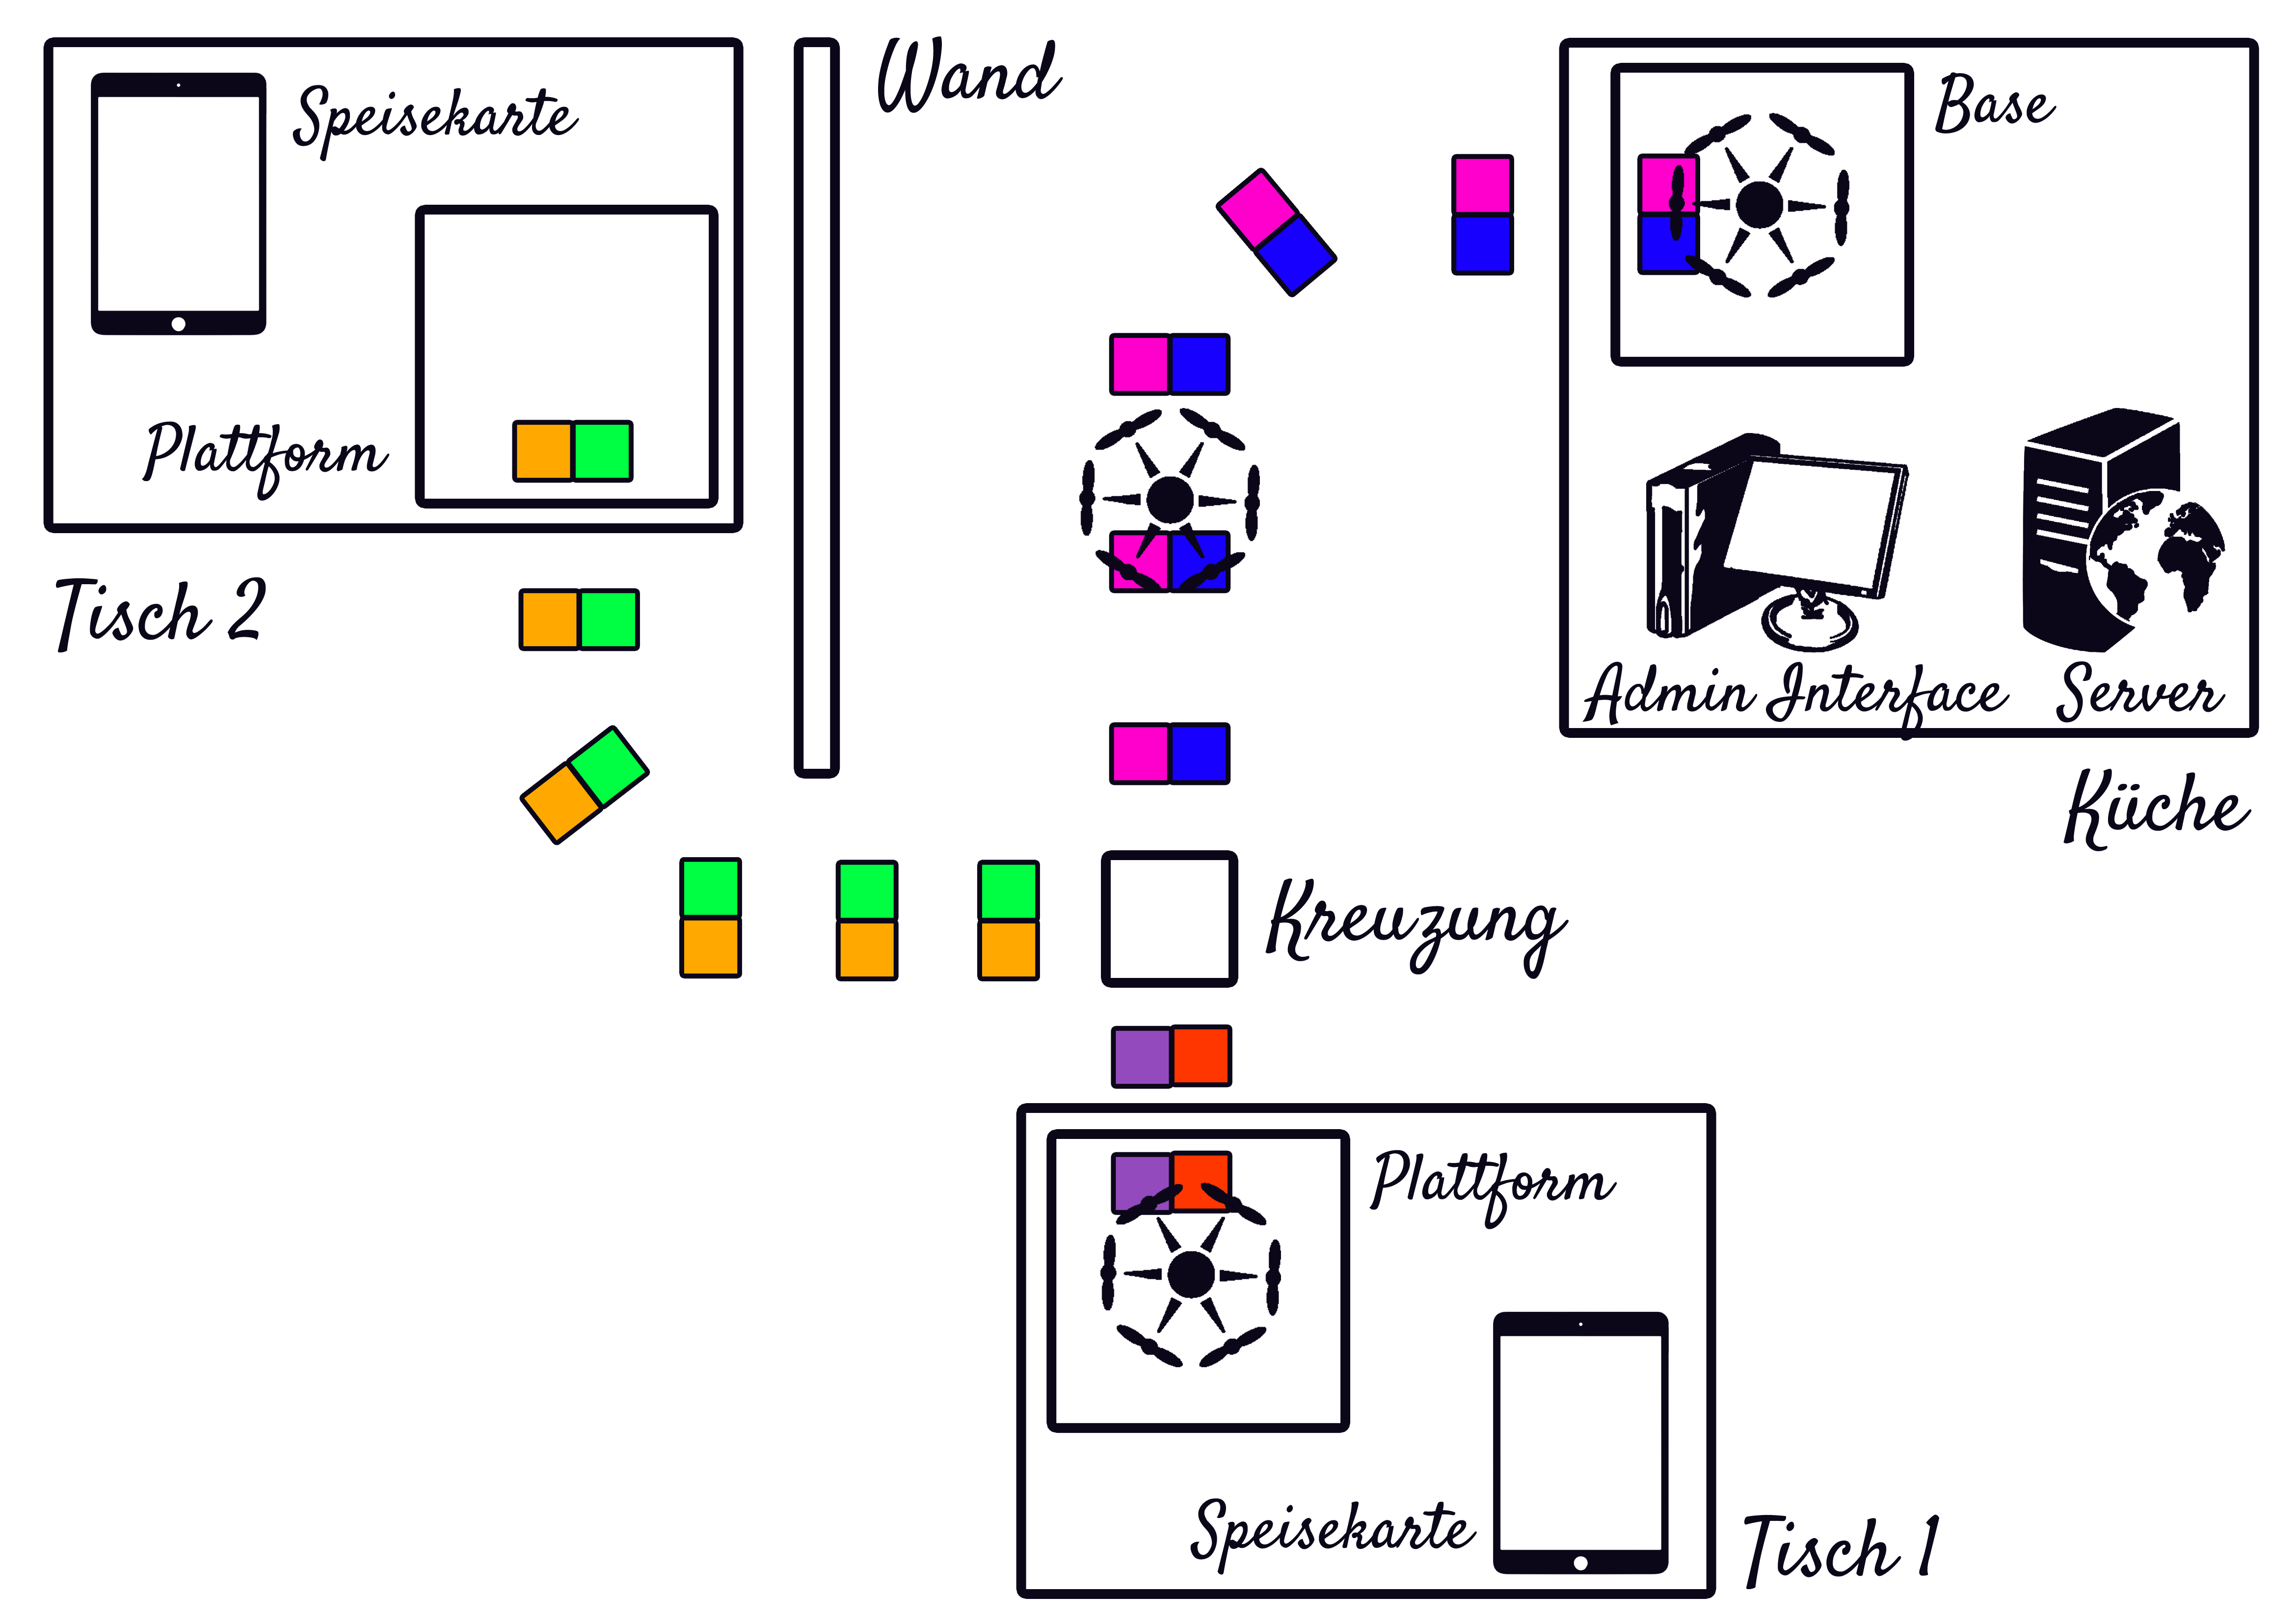
\includegraphics[width = 100mm]{Bilder/Ablauf}
\par\end{centering}
\caption{Der Weg einer Bestellung}
\label{Ablauf}
\end{figure}

%%%%Systemblockbild
\begin{figure}[tbh]
\begin{centering}
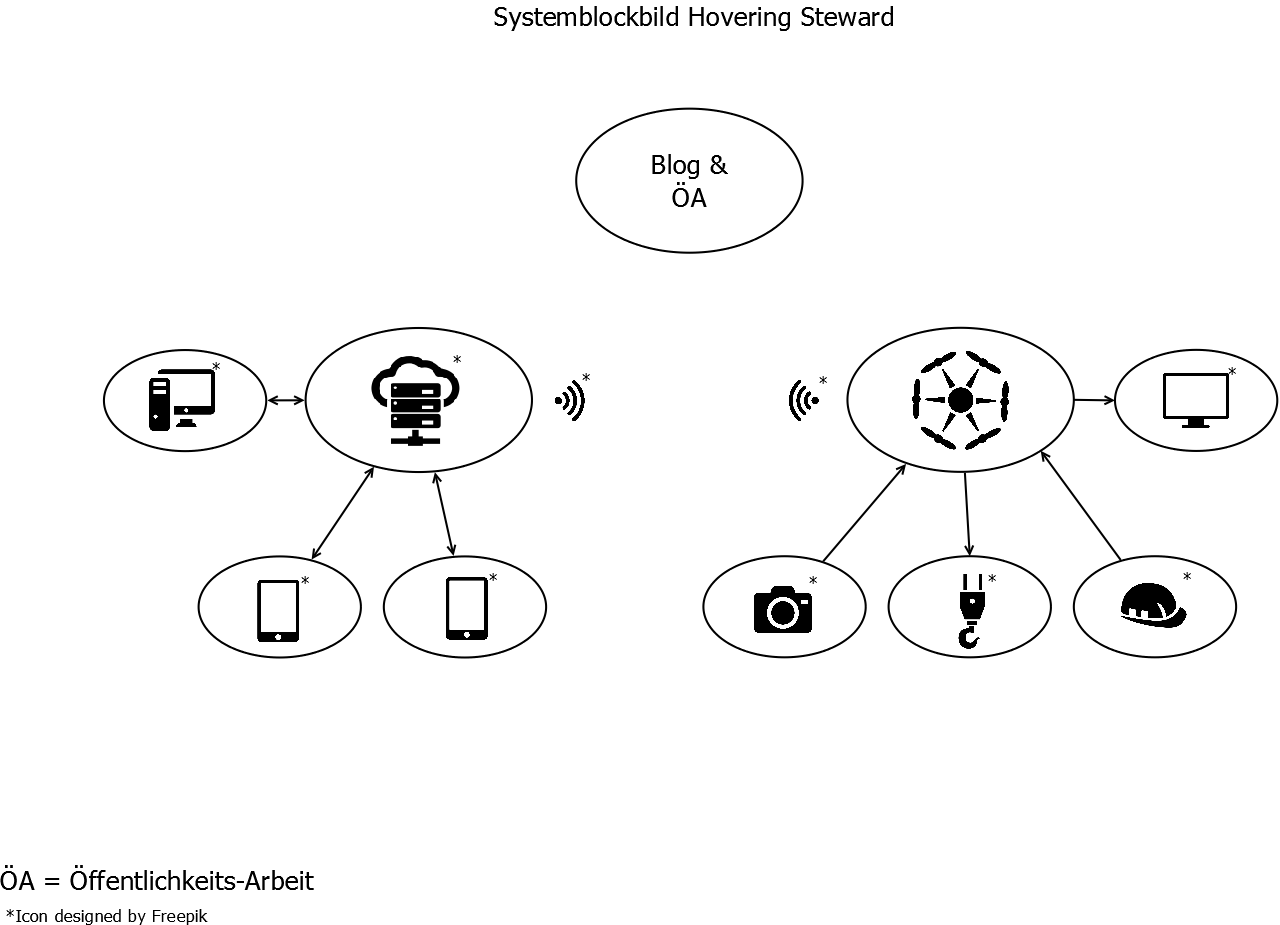
\includegraphics[angle = 90, width = \textwidth]{Bilder/Systemblockbild}
\par\end{centering}
\caption{Das Zusammenwirken der Komponenten}
\label{Systemblockbild}
\end{figure}